\documentclass[times, utf8, seminar, numeric]{fer}
\usepackage{booktabs}
\usepackage{url}

\usepackage{graphicx}  				% Versatile graphics manipulation options
\usepackage[font=footnotesize]{subfig}

\usepackage[croatian]{babel}  % Croatian typographical rules and hyphenation patterns 
\usepackage[utf8]{inputenc}  	% Encoding of Croatian characters
\usepackage[T1]{fontenc}
\usepackage{ae,aecompl}     	% Type 1 fonts, similar to Computer Modern (Comment this line for Times New Roman)
\usepackage{hyperref}
\hypersetup{
    colorlinks=true,
    linkcolor=black,
    filecolor=magenta,      
    urlcolor=blue,
}
\usepackage{microtype}				% Improves spacing

\begin{document}
\setcounter{secnumdepth}{3} 
\setcounter{tocdepth}{4}
% Ukljuci literaturu u seminar
\nocite{*}

\title{LPWAN: LoRa}

\author{Krešimir Topolovec}

\voditelj{Doc. dr. sc. Igor Čavrak}

\maketitle

\tableofcontents

\chapter{Uvod}
\label{chapter:uvod}
Gotovo uvijek u realnom svijetu imamo slučaj da su resursi ograničeni. U svijetu elektroničkih komunikacija resurse predstavljaju električna energija, a u bežičnim komunikacijama još je bitan i faktor dostupnosti radio-frekvencijskog spektra. Napretkom tehnologije, na svijetu se generira sve veća količina podataka te raste potreba za prijenosom tih podataka, a još k tome raste i broj sudionika u komunikacijskim mrežama. Sve te činjenice guraju dalje razvoj komunikacijskih tehnologija, a prije svega bežičnih odnosno mobilnih tehnologija pred koje se stavljaju sve veći izazovi.
\newline

Kada govorimo o bežičnim komunikacijima prvo nam na pamet padaju mobilne mreže 3. i 4. generacije (3G i LTE) ili WiFi (IEEE 802.11 a/b/g/n/ac) bežična tehnologija koja se koristi unutar LAN mreža. Takve tehnologije omogučavaju prijenos velike količine podataka, za današnje pojmove velikom brzinom. Nedostatak ovih tehnologija i uređaja koji koriste ove tehnologije je relativno velika potrošnja električne energije. To je između ostalog jedan od razloga zašto današnje mobilne uređaje, pametne telefone i ostale baterijski napajane uređaje svakog dana moramo spajati na punjenje. Usmjerivači i slični mrežni uređaji ne mijenjaju položaj te stoga pristup električnoj energiji za takve primjere uređaja ne predstavlja problem.
\newline

Međutim, postoje uređaji koji moraju mjesecima ili čak godinama raditi bez mogučnosti trajnog iskorištavanja električne energije iz gradske mreže ili svakodnevnog punjenja. Logičan način za napajanje takvih uređaja je baterija i/ili manji solarni panel ili sličan način prikupljanja energije iz okoline odnosno iskorištavanja obnovljivih izvora energije. Takvi baterijski napajani uređaji, kako bi dugo mogli obavljati svoju funkciju, moraju trošiti iznimno malo električne energije, a istovremeno imaju potrebu za bežičnom komunikacijom koja redovno troši najviše energije. Uređaji s takvim potrebama zahtjevaju specifičnu komunikacijsku tehnologiju i protokol.
\newline

LPWAN (Low-Power Wide-Area Network) je bežična komunikacijska tehnologija koja je dizajnirana da omoguči komunikaciju na velike udaljenosti, uz malu potrošnju električne energije, između uređaja koji generiraju manje količine podataka (npr. senzori koji rijetko mjere spore promjene fizikalne veličine koja se mjeri). Jedna od najzastupljenijih LPWAN tehnologija je LoRa koja će detaljnije biti opisana u poglavlju \ref{chapter:lora}.
\chapter{LPWAN}
\label{chapter:lpwan}

LPWAN (Low-Power Wide-Area Network) je tehnologija za bežičnu komunikaciju na širokom području uz nisku potrošnju električne energije. Zbog zahtjeva za komunikacijom u M2M (Machine to Machine) i IoT (Internet of Things) sustavima razvijaju se mnoge LPWAN tehnologije te su dokaz današnjeg trenda evolucije telekomunikacija. Fokus ovog rada je jedna od tih tehnologija.
\newline

\section{Karakteristike}
\label{section:lpwan_karakteristike}
Komunikacija niske potrošnje energije uz nižu cijenu tehnologije u odnosu na slučaj sa tradicinonalnim mobilnim mrežama jedan je od aduta LPWAN tehnologija. Također i podrška za veći broj spojenih uređaja na većem geografskom području.
\newline
Tipične veličine paketa u LPWAN-u su između 10B i 1kB uz brzine prijenosa do 200kbps. Najčešća topologija u ovakvim mrežama je zvijezdasta gdje se krajnje točke spajaju na zajedničku pristupnu točku kao i kod WiFi tehnologije.
\newline

Neke od najpoznatijih LPWAN tehnologija su: \begin{itemize}
\item Sigfox
\item Lora
\item NB-IoT (Narrowband-IoT)
\item LTE-M
\item Nwave
\item RPMA
\end{itemize}

\begin{figure}[ht!]
\centering
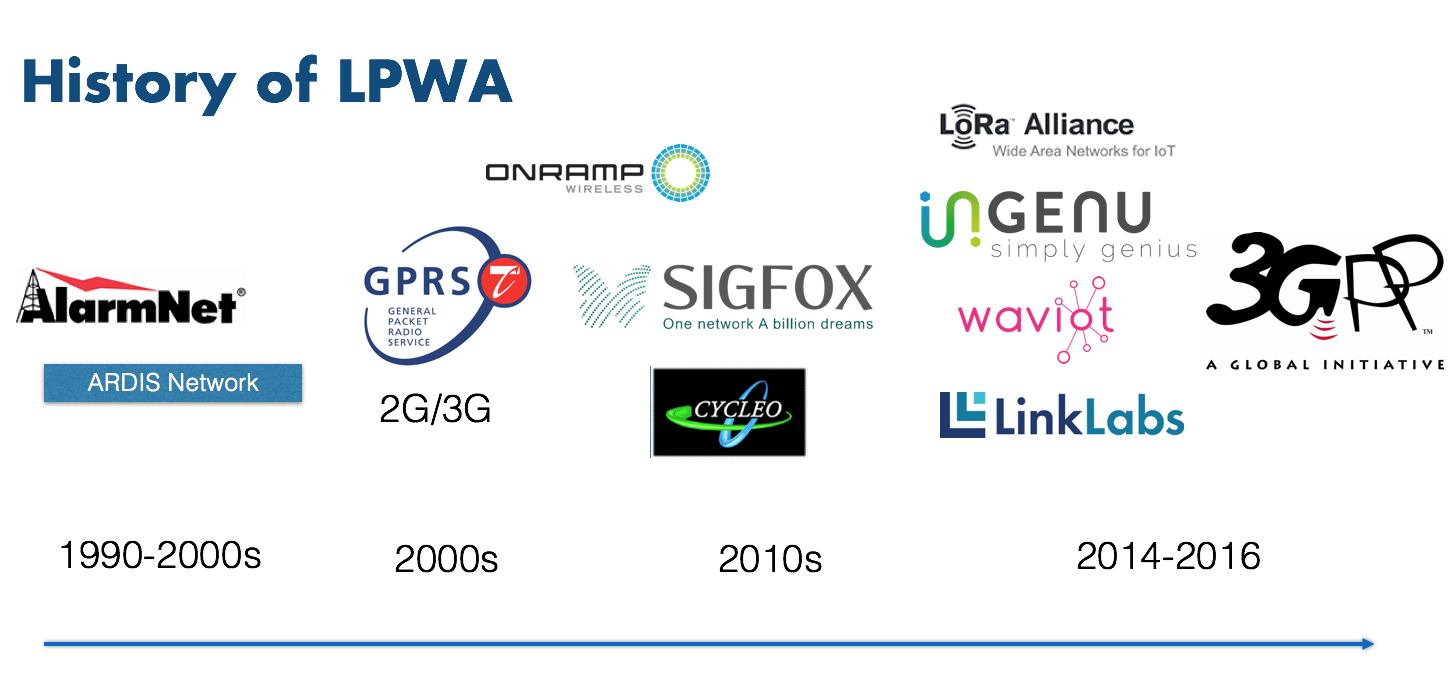
\includegraphics[width=1.0\textwidth]{images/lpwan_history.png}
\caption{Pregled LPWAN tehnologija kroz povijest}
\label{img:lpwan_overview}
\end{figure}

\pagebreak
S obzirom na velik broj raspoloživih tehnologija gdje svaka nudi nešto drugačije teško je ili nemoguće reći koja je najbolja. Možemo predpostaviti da će potrebe IoT-a i ostalih primjena dalje pogoniti razvoj te da će se kroz par godina iskristalizirati situacija među morem raspoloživih tehnologija.
Pri odabiru tehnologije za konkretnu primjenu odnosno projekt potrebno je svakako sagledati sve prednosti i mane pojedine tehnologije.
\newline

Najbitnije karakteristike LPWAN mreža:
\begin{itemize}
\item Mala potrošnja električe energije - omogućuje dugotrajan rad baterijski napajanih uređaja (do 10 ili više godina)
\item Komunikacija na velike udaljenosti
\item Moguć velik broj sudionika u mreži (visok kapacitet mreže)
\item Potrebno malo baznih stanica (u odnosu na mobilne mreže)
\item Korištenje uglavnom nelicenciranog spektra (LoRa i Sigfox)
\item Niska cijena komunikacijskih modula/chipseta (mala kompleksnost sklopovlja)
\item Niska latencija
\end{itemize}

\vspace{5mm}
Najčešći zahtjevi M2M i IoT sustava, a koji nisu dobro podržani tradicionalnim tehnologijama su potreba za komunikacijom na velike udaljenosti i na velikom području te najčešće prijenos male količine podataka te vrlo mala frekvencija slanja ili primanja podataka (čak do samo par poruka dnevno).
Ovi zahtjevi uzeti su u obzir pri dizajniranju LPWAN tehnologija. Kako bi navedeni zahtjevi mogli biti zadovoljeni napravljen je kompromis na štetu brzine prijenosa podataka, što za M2M i IoT primjene najčešće nije problem zbog male količine podataka koju je potrebno prenjeti.
Usporedba LPWAN mreže s ostalim mrežama prikazana ja na slici \ref{img:comparison}.
\begin{figure}[ht!]
\centering
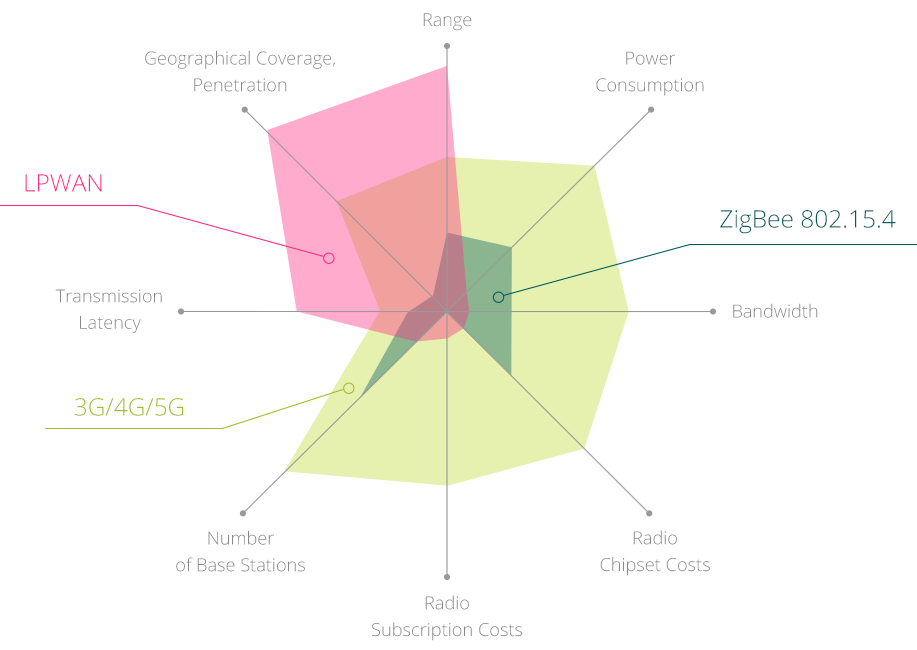
\includegraphics[width=1.0\textwidth]{images/lpwan_other_comparison.png}
\caption{Usporedba bežičnih komunikacijskih mreža}
\label{img:comparison}
\end{figure}

\section{Primjena}
\label{section:lpwan_primjena}
Moguća područja za primjenu neke od LPWAN tehnologija su sva gdje je potreban prijenos male količine podataka na velike udaljenosti uz minimalnu potrošnju električne energije odnosno minimalnu potrošnju baterije ako su krajnji uređaji napajani baterijski.

\pagebreak
Područja primjene i neki aktualni primjeri:
\begin{itemize}
\item Pametni gradovi (pametni semafori, pametna rasvjeta i sl.)
\item Transport
\item Precizna poljoprivreda (npr. određivanje idealnog trenutak za sjetvu ili praćenje parametara tla)
\item Senzorske mreže
\item Telemedicina
\item Praćenje parametara iz prirode (npr. predviđanje potresa i zagađenja zraka)
\item Praćenje parametara infrastrukture (npr. mostovi i tuneli)
\end{itemize}


\begin{figure}[ht!]
\centering
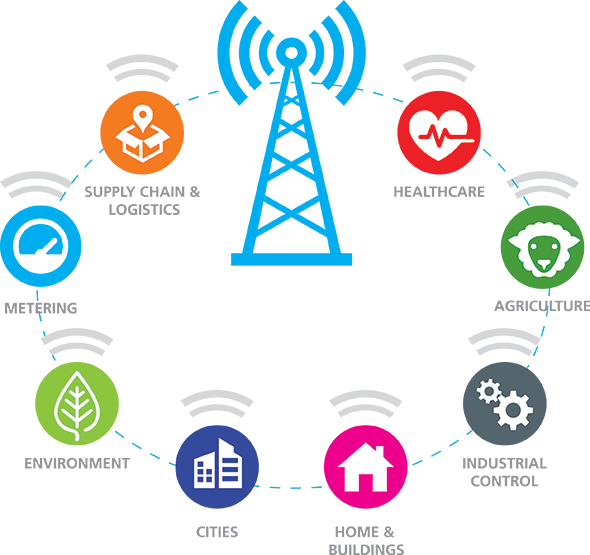
\includegraphics[width=0.8\textwidth]{images/use_cases.png}
\caption{Područja primjene LPWAN tehnologija}
\label{img:comparison}
\end{figure}


\chapter{LoRa}
\label{chapter:lora}
LoRa (engl. Long Range) je patentirana tehnologija za bežičnu komunikaciju na velike udaljenosti za uređaje s ograničenom energijom. Prvotno je razvijena od strane tvrtke Cycleo, a danas ju razvija i patentirana je od strane tvrtke \href{https://www.semtech.com}{Semtech}. Osim tvrtke Semtech, u razvoj su uključene i tvrtke Actility  i IBM.

\section{Osnovne karakteristike}
\label{subsection:osnovno}
\begin{itemize}
\item LoRa omogućuje komunikaciju na udaljenostima većim od 10km u ruralnim područjima i nekoliko kilometara u urbanim područjima
\item Mala potrošnja električne energije - moguće postići trajanje baterije od nekoliko godina
\item Prijenos male količine podataka
\item Mala brzina prijenosa podataka
\item Robustan komunikacijski protokol - otpornost na smetnje
\item Korištenje komunikacijskog kanala 1\% vremena ili manje (eng. Duty Cycle) - podaci se ne šalju visokom frekvencijom tj. koristi se tzv. burst način prijenosa
\item Visok kapacitet mreže - moguća komunikacija velikog broja krajnjih uređaja, na jednu baznu stanicu moguće spojiti do 20 000 uređaja
\item  LoRa za komunikaciju koristi uglavnom nelicencirani radio-frekvencijski spektar (npr. 868MHz u Europi ili 915Mhz u Sjevernoj Americi)
\item LoRa implementira sigurnost u dva sloja
\item Više načina rada krajnjih uređaja - klase A, B i C
\item Mogučnost stvaranja privatnih i javnih mreža
\item Jednostavno integriranje u postojeću infrastrukturu
\item Mogučnost geolokacije bez prisutnosti GPS tehnologije
\end{itemize}

\section{LoRa stog}
\label{section:lora_overview}
Kada govorimo o LoRa tehnologiji bitno je razlikovati dva segmenta. Prvi dio LoRa-e definira modulacijski postupak, frekvencije i ostale parametre fizičkog sloja. Fizički sloj nije otvoreno rješenje jer tvrtka Semtech drži patente na postupak modulacije. Drugi segment, LoRaWAN, definira komunikacijski protokol i arhitekturu mreže. LoRaWAN je također i standard i specifikacija koju razvija i promovira \href{https://lora-alliance.org/}{LoRa alijansa}. Fizički sloj LoRa tehnologije možemo promatrati kao prvi sloj, a LoRaWAN možemo promatrati kao drugi i treći sloj referentnog \href{https://en.wikipedia.org/wiki/OSI_model}{OSI} modela.

\begin{figure}[ht!]
	\centering
	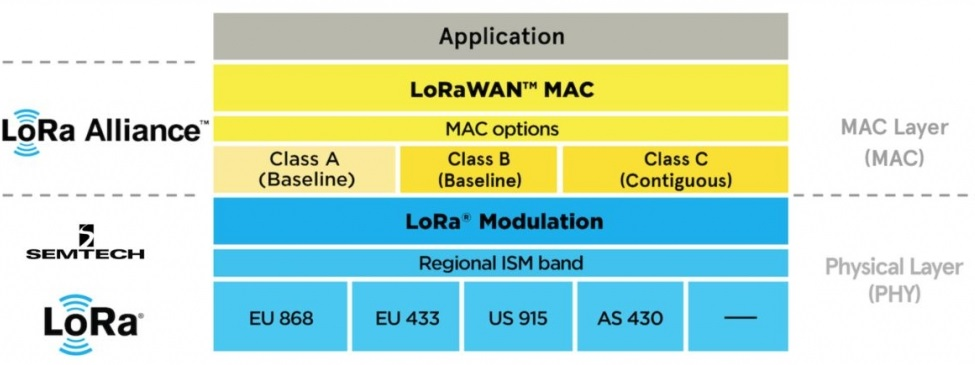
\includegraphics[width=1.0\textwidth]{images/lorawan-stack.jpg}
\caption{Struktura LoRa slojeva - LoRa stog}
\label{img:lora_stack}
\end{figure}



\section{LoRa fizički sloj}
\label{section:lora_phy}
Fizički sloj definira sve što je neophodno da bi se uspostavila komunikacija radio-frekvencijskim spektrom i višim slojevima omogućilo korištenje komunikacijskog kanala. 
Bitni segmenti fizičkog sloja razjašnjeni su u slijedećim potpoglavljima. Poznavanje karakteristika modulacijskog postupka i ostalih bitnih dijelova fizičkog sloja je nužno za razumijevanje prednosti i mana LoRa tehnologije.

\subsection{Modulacijski postupak}
\label{subsection:lora_modulation}
Modulacijski postupak definira postupak korištenja energije elektromagnetskog vala i dijela elektromagnetskog spektra kako bi se prenjela informacija.\newline
LoRa kao modulacijski postupak koristi derivat modulacije raspršenog spektra, tzv. CSS modulacijski postupak (eng. Chirp Spread Spectrum). U LoRa modulaciji se koriste tzv. chirp-ovi kod kojih frekvencija linearno raste ili pada između granica frekvencijskog pojasa (eng. bandwidth - \textbf{BW}) na kojem se komunikacija odvija. Raspršenje spektra zapravo je ostvareno tim porastom ili padom frekvencije chirp-ova. Ovisno o rastu ili padu frekvencije razlikujemo up-chirp (slika \ref{img:up_chirp}) i down-chirp. Postoje i druge varijante chirp-ova kod kojih se frekvencija mijenja nelinearno no takvi nisu korišteni u LoRa modulaciji. S obzirom da je CSS modulacija razvijena za primjenu u radarima, naziv \textit{chirp} dolazi od engleskog naziva \textit{Compressed High Intensity Radar Pulse}. CSS modulacija se također dugi niz godina koristi za komunikaciju u vojnim i svemirskim sustavima. LoRa je prva cjenovno prihvatljiva implementacija takve tehnologije namjenjena za komercijalne primjene.
\begin{figure}[ht!]
	\centering
	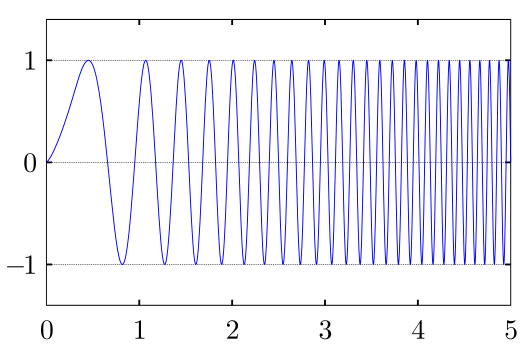
\includegraphics[width=0.65\textwidth]{images/linear_chirp.png}
	\caption{Amplitudno-vremenska karakteristika jednog up-chirp impulsa}
	\label{img:up_chirp}
\end{figure}
\begin{figure}[ht!]
	\centering
	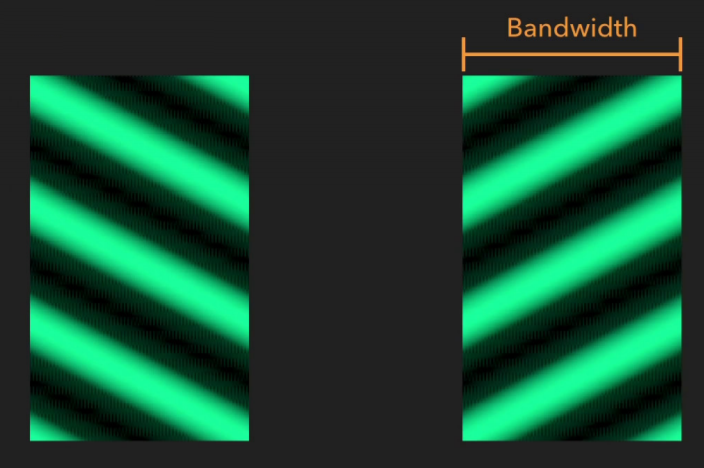
\includegraphics[width=0.65\textwidth]{images/chirps.png}
	\caption{Vodopadni prikaz nekoliko linearnih up-chirp (lijevo) i down-chirp (desno) impulsa }
	\label{img:chirps}
\end{figure}

\newpage
\begin{subsubsection}{Teorijska pozadina}
\label{subsubsection:therory}
Radi boljeg razumijevanja LoRa tehnologije dobro je poznavati slijedeće definicije i iskaze.

\paragraph{Teorem Shannon–Hartley}\mbox{}\\
Teorem definira maksimalnu brzinu $\mathbf{C} [b/s]$ kojom se podaci mogu prenositi komunikacijskim kanalom na definiranom pojasu \textbf{BW} [Hz] uz prisutnost šuma \textbf{N} [W] i snagu signala \textbf{S} [W].
\begin{equation}
C = BW log_{2}(1 + \frac{S}{N}) \quad [b/s]
\label{eq:shannon_hartley}
\end{equation}
Ako u izrazu \ref{eq:shannon_hartley} napravimo aproksimaciju, pretvorimo $log_2$ u $ln$ i koristimo da je $\frac{1}{ln2}= 1.443$, možemo ga zapisati kao:
\begin{equation}
  \frac{C}{BW} = 1.443 \frac{S}{N}
  \label{eq:shannon_hartley_2}
\end{equation}
Iz dobivenog izraza je vidljivo da je za konstantni odnos signal/šum ($\mathbf{S/N}$) potrebno povećati pojas \textbf{BW} kako bi se postigao veći kapacitet komunikacijskog kanala \textbf{C}, odnosno kako bi se postigla  veća brzina.
S obzirom da je u modulaciji raspršenog spektra odnos \textbf{S/N} redovno manji od 1 ili negativan u decibelima, to se kompenzira širim pojasom \textbf{BW} kako bi se zadržao potreban kapacitet komunikacijskog kanala odnosno ostvarila potrebna brzina.

\paragraph{FSPL (Free Space Path Loss)}\mbox{}\\ 
FSPL je faktor koji definira gubitak energije radio signala između dvije antene udaljene za $d$ u slobodnom prostoru. Intuitivno je jasno da uz manji gubitak energije signala moguće postići komunikaciju na veće udaljenosti. FSPL je definiran s izrazom:
\begin{equation}
  FSPL = (\frac{4\pi d}{\lambda})^2 
  \label{eq:fspl}
\end{equation}
S obzirom da se radi o elektromagnetskim valovima, izraz \ref{eq:fspl} se može zapisati kao:
\begin{equation}
  FSPL = (\frac{4\pi d f}{c})^2 
\end{equation}
gdje je $f$ frekvencija, a $c$ konstantna brzina svjetlosti.

Prikladniji način za prikaz gubitka energije RF signala je u logaritamskom obliku:
\begin{equation}
\begin{gathered}
FSPL = 20 log_{10}(d) + 20 log_{10}(f) + 20 log_{10}(\frac{4 \pi}{c})
\\
= 20 log_{10}(d) + 20 log_{10}(f) - 147.56
\end{gathered}
\label{eq:fspl_3}
\end{equation}
Bitno je napomenuti da ovi izrazi vrijede u slobodnom prostoru. U realnim situacijama, gdje signal na svom putu prolazi kroz razne prepreke kao što su beton, voda, zrak, staklo i sl. gubici su još veći. Gornjim jednostavnim izrazom moguće je u grubo aproksimirati gubitke energije signala. Možemo biti sigurni da gubici u realnim uvjetima nikako neće biti manji od FSPL gubitaka, te tako barem odrediti jedan rubni slučaj. Maksimalne gubitke je nemoguće odrediti s obzirom da oni ovise o okolini.
Za istu udaljenost i uz dvije različite frekvencije, gubici su za nižu frekvenciju manji. LoRa radi na frekvencijama nižim od 1GHz. Ako usporedimo FSPL gubitke na nekoj LoRa frekvenciji (u primjeru 868MHz EU frekvencija) i gubitke na 2,4GHz, što je frekvencija na kojoj rade WiFi i Bluetooth tehnologije, uočiti ćemo jedan od razloga zbog kojeg LoRa omogućuje komunikaciju na velike udaljenosti.
\begin{equation}
\varDelta{FSPL} = |FSPL_{868MHz} - FSPL_{2,4GHz}| \approx 9dB
\label{eq:fspl_delta}
\end{equation}

\paragraph{Osjetljivost prijamnika}\mbox{}\\
Osjetljivost prijamnika $\mathbf{S}$ je najniža razina primljene snage na kojoj je prijamnik može detektirati RF signal i iz njega demodulirati podatke. Osjetljivost prijamnika je iznimno bitna karakteristika prijamnika u svakoj bežičnoj komunikaciji. Niža osjetljivost znaći bolji prijam slabih signala odnosno veći doseg komunikacije.

Osjetljivost RF prijamnika dana je formulom:
\begin{equation}
\begin{aligned}
&S = -174 + 10log_{10}(BW) + NF + S/N \quad [dB]
\\
&BW[Hz] \text{ - širina pojasa}\\
&NF[dB] \text{ (Noise Figure) - faktor koji ovisi o implementaciji prijamnika} \\
&S/N[dB] \text{ - odnos signal/šum}
\end{aligned}
\end{equation}
\begin{figure}[ht!]
	\centering
	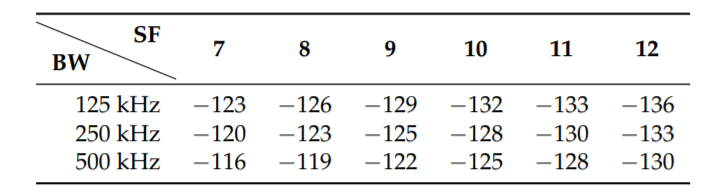
\includegraphics[width=0.6\textwidth]{images/sx1276.png}
	\caption{Ovisnost osjetljivosti Semtech SX1276 prijamnika o parametrima SF i BW}
	\label{img:sx1276sensitivity}
\end{figure}

\end{subsubsection}


\subsection{Karakteristike LoRa modulacije}
\label{subsection:lora_mod_params}

Prije detaljnije razrade LoRa modulacije potrebno je definirati neke parametre:
\begin{itemize}
\item Frekvencijski pojas (eng. Bandwidth) $\mathbf{BW} [Hz]$ - dio spektra nad kojim se odašilju/primaju podaci, odnosno vrši raspršenje
\item Faktor širenja (eng. Spreading Factor) - $\mathbf{SF} [\frac{chip}{simbol}] \in 7..12$
\item Trajanje LoRa simbola - $\mathbf{T_{symbol}} [s]$
\item Brzina slanja simbola - $\mathbf{R_{symbol}} [simbol/s]$
\item Brzina slanja bitova infromacije - $\mathbf{R_{bit}} [b/s]$
\item Brzina slanja chip-ova - $\mathbf{R_{chip}} [chip/s]$
\item Code Rate $\mathbf{CR}$ - udio redundantnih bitova $\in \frac{4}{5} .. \frac{4}{8} $
\item Izračena snaga - $\mathbf{P_{TX}} \in -4...20dBm$ 
\end{itemize}

\vspace{10px}
\noindent
U digitalnim komunikacijama, simbol kodira jedan ili više bitova podataka. Trajanje LoRa simbola definirano je izrazom:
\begin{equation}
  T_{symbol} = \frac{2^{SF}}{BW}
  \label{eq:symbol_time}
\end{equation}
Recipročna vrijednost trajanja simbola daje nam izraz za brzinu slanja LoRa simbola (eng. Symbol Rate):
\begin{equation}
 R_{symbol} = \frac{1}{T_{symbol}}
 \label{eq:symbol_rate}
\end{equation}
SF parametar također određuje broj tzv. chip-ova po simbolu.
Chip je puls, možemo ga promatrati kao bit u kontekstu modulacije. Ideja je svaki bit informacije raspršiti spektrom BW slanjem $2^{SF}$ chip-ova za svaki simbol.
Možemo definirat parametar $R_{chip}$ (Chip Rate):
\begin{equation}
R_{chip} = 2^{SF} R_{symbol}
\end{equation}
Rasprešene informacije, tj. tok chip-ova, LoRa šalje brzinom koja je jedanaka širini spektra BW. Dakle, za 125 kHZ, $R_{chip}$ će biti 125 000 chip-ova u sekundi.
\begin{equation}
\begin{gathered}
R_{chip} = 2^{SF} R_{symbol} = 2^{SF} \frac{BW}{2^{SF}} = BW
\\
T_{chip} = \frac{1}{BW}
\end{gathered}
\end{equation}
Obzirom da se za svaki simbol šalje $2^{SF}$ chip-ova, izraz \ref{eq:symbol_time} sada možemo zapisati kao:
\begin{equation}
T_{symbol} = 2^{SF} T_{chip} = \frac{2^{SF}}{BW}
\end{equation}
U LoRa modulaciji svaki simbol kodira $SF$ bitova podataka pa možemo izvesti slijedeći izraz za brzinu prijenosa bitova:
\begin{equation}
\begin{gathered}
R_{bit} = {SF} * R_{symbol}
\\
R_{bit} = SF \frac{BW}{2^{SF}}
\end{gathered}
\label{eq:r_bit}
\end{equation}
Iz dobivenog izraza \ref{eq:r_bit} je jasno da brzina prijenosa podataka direktno ovisi o faktoru SF te širini spektra BW. Za odabrani spektar BW postiže se veća brzina prijenosa za manji SF.
\begin{equation}
\begin{gathered}
R_{bit} = 6835 bps \text{ za } SF = 7\text{, }  BW = 125 kHz
\\
R_{bit} = 366 bps \text{ za } SF = 12\text{, } BW = 125 kHz
\end{gathered}
\end{equation}

\noindent
Na slici \ref{img:demodulation} je ilustrirana modulacija i kodiranje nekoliko LoRa simbola. 	
\begin{figure}[ht!]
	\centering
	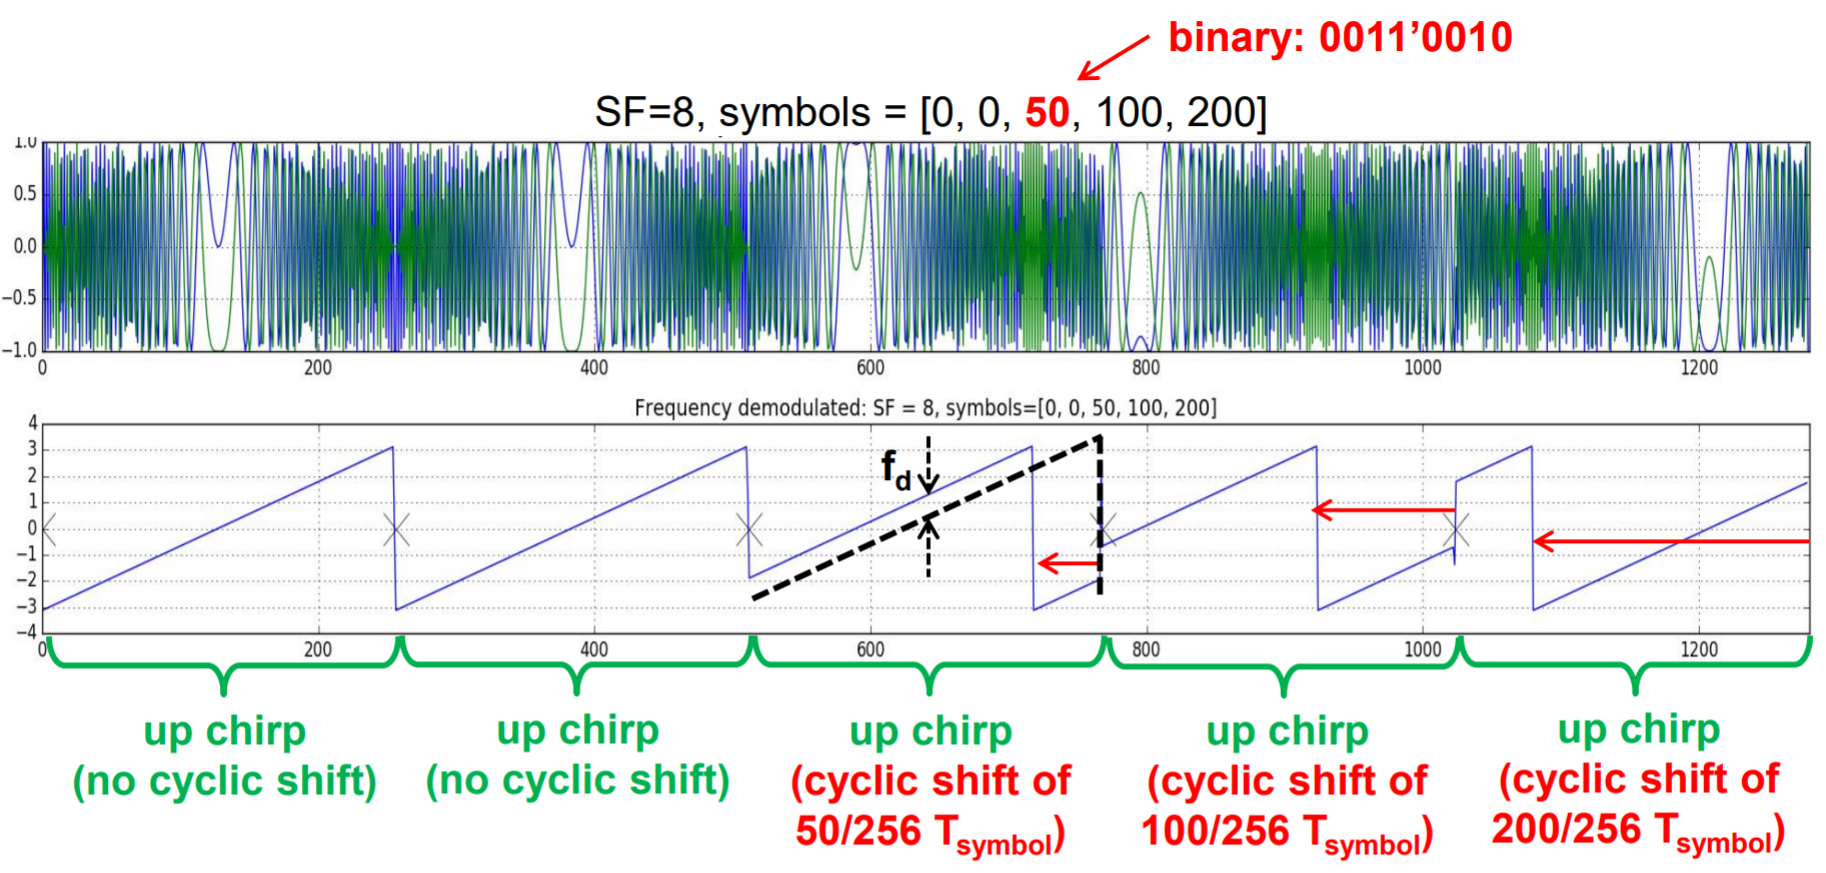
\includegraphics[width=1.0\textwidth]{images/demodulation.png}
	\caption{Modulacija i kodiranje LoRa simbola}
	\label{img:demodulation}
\end{figure}
Odabrani SF je 8, dakle svaki LoRa simbol kodira 8 bitova podataka što je i prikazano na slici. Svaki simbol je moduliran sa $2^{SF}$ chip-ova, u ovom slučaju 256. Kodirani niz simbola je $ [0,0,50,100,200]$. Cikličkim posmakom chirp-a ostvaruje se moduliranje konkrentog simbola. Na primjer, za simbol 50, chirp je posmaknut za $50/256$ trajanja samog simbola $T_{symbol}$ u lijevo. Razlika u frekvenciji između posmaknutog i neposmaknutog chirp-a koju detektira LoRa prijamnik je na slici označena s $f_{d}$. Referentni neposmaknutni chirp-ovi poslani su na početku LoRa okvira (\ref{subsection:lora_frame})

\paragraph*{FEC}\mbox{}\\ 
\label{paragraph:fec}
LoRa zbog pouzdanosti prijenosa podataka koristi mehanizam ispravljanja greške u primljenim bitovima (eng. Forward correction code - FEC). Zbog redundantnih bitova, na strani prijamnika moguće je otkriti grešku koja se desila tokom prijenosa. Mehanizam donosi veću pouzdanost prijenosa, ali smanjuje brzinu prijenosa korisnih podataka. LoRa nudi mogučnost odabira u kojoj mjeri želimo koristiti mehanizam FEC, parametrom CR (eng. Code Rate).
\begin{equation}
CR = \frac{4}{4 + n} ,\quad n \in 1..4
\end{equation}
Brzina prijenosa sada je:
\begin{equation}
R_{bit} = SF \frac{BW}{2^{SF}} CR = SF \frac{BW}{2^{SF}} \frac{4}{4+n}
\end{equation}
\\
Na slici \ref{img:chirps_comparison_sf} prikazana je razlika u trajanju chirp-ova tj. simbola za različite vrijednosti parametra SF. 
\begin{figure}[ht!]
	\centering
	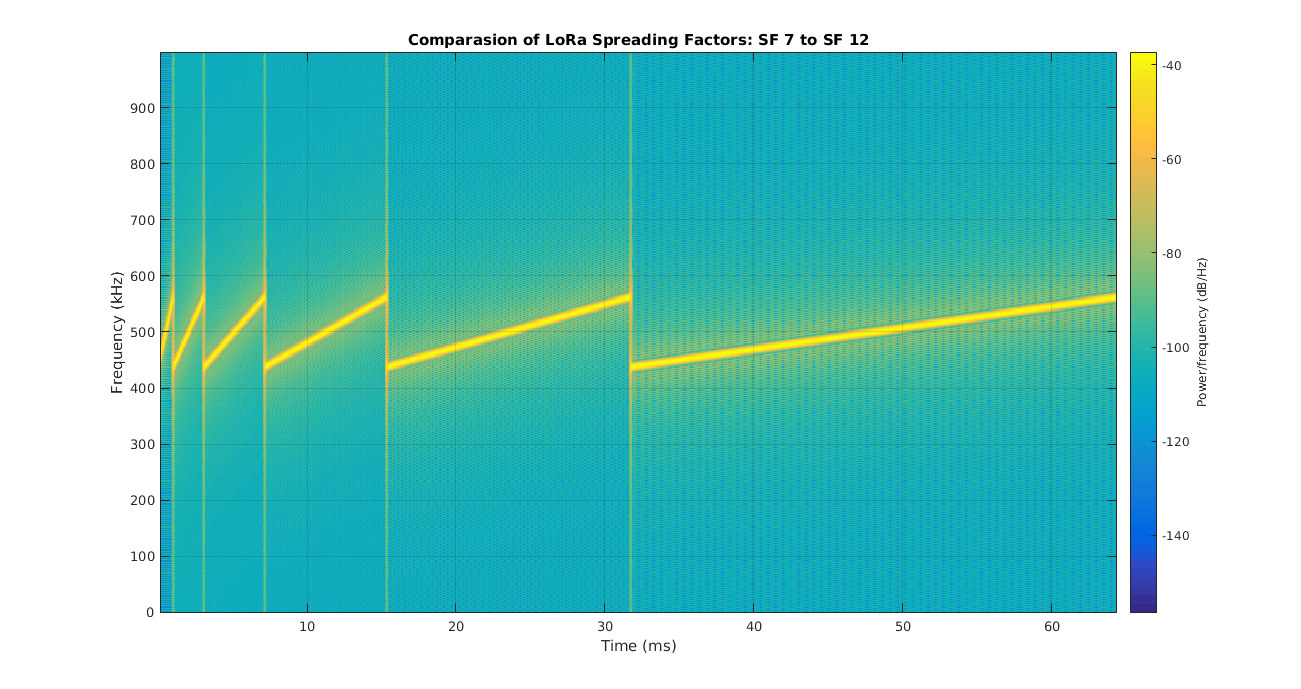
\includegraphics[width=0.9\textwidth]{images/SF_Comparasion_7_12.png}
	\caption{Usporedba chirp-ova za razne vrijednosti parametra SF}
	\label{img:chirps_comparison_sf}
\end{figure}

\noindent
Raspršenjem podataka po spektru ostvaruje se tzv. dobitak pri procesiranju (eng. Processing Gain $\mathbf{G_{p}})$. Processing Gain je svojstvo svih Spread Spectrum modulacija.
\begin{equation}
\begin{gathered}
G_{p} = 10 \log_{10}(\frac{R_{chip}}{R_{bit}}) \quad[dB]\\
= 10 \log_{10}(\frac{BW}{SF\frac{BW}{2^{SF}}})\\
= 10 \log_{10}(\frac{2^{SF}}{SF}) \quad[dB]
\label{eq:pgain}
\end{gathered}
\end{equation}

\noindent
Većim dobitkom pri procesiranju moguće je ostvariti veći domet komunikacije. Iz izraza \ref{eq:pgain} vrijedi da za veći faktor raspršenja $\mathbf{SF}$ ostvarujemo veću dobit pri procesiranju, a time i veći domet komunikacije.

Bitno je napomenuti da za veći $\mathbf{SF}$ duže traje prijenos pojedinog simbola pa i prijenos svih podataka što na kraju rezultira dužom aktivnosti samog LoRa uređaja (eng. Time on Air), a time se troši više energije koja je često strogo ograničena u aplikacijma u kakvima se koristi LoRa tehnologija.
\newline

Možemo zaključiti glavne karakteristike vezane uz parametar $\mathbf{SF}$:
\begin{itemize}
\item ključan parametar u određivanju brzine prijenosa i udaljenosti tj. dosega komunikacije - SF parametar zapravo predstavlja kompromis između brzine prijenos podataka i dosega komunikacije
\item broj podatkovnih bitova kodiranih pojedinim simbolom jednak je $SF$
\item određuje trajanje simbola $T_{symbol}$
\item utječe na trajanje prijenosa podataka (eng. Time On Air)
\item broj chip-ova sadržanih u svakom simbolu jednak je $2^{SF}$
\end{itemize}

\subsection{Link Budget}
\label{subsection:link_budget}
Link Budget bi se možda mogao prevesti kao budžet komunikacijskog kanala. To je zapravo razlika između efektivne izračene snage na predajniku i osjetljivosti prijamnika. Efektivna izračena snaga predajnika (na slici \ref{img:link_bduget} EIRP) je sama izračena snaga predajnika umanjena za gubitke u kabelu i konektorima te uvećana za dobitak antene predajnika. Na strani prijamnika također se ostvaruje dobitak antenom i gubitak snage u konektorima i kabelu. Ostatak snage signala potrošen je pri prijenosu signala kroz medij (pogledati potpoglavlje \ref{subsubsection:therory} i FSPL). Svi gubici $L$, dobici $G$ i snage $P$ na prijamniku RX i predajniku TX povezani su slijedećom relacijom:
\begin{equation}
\begin{aligned}
&P_{RX} = P_{TX} + G_{TX} - L_{TX} - L_{FS} - L_{M} + G_{RX} - L_{RX} \quad[dB] \\
&P_{RX} \text{ - snaga na prijamniku}\\
&P_{TX} \text{ - snaga na predajniku}\\
&G_{TX} \text{ - dobitak (gain) predajne antene}\\
&L_{TX} \text{ - gubici predajnika (kabel, konektori...)}\\
&L_{FS} \text{ - gubici u mediju (pogledati potpoglavlje \ref{subsubsection:therory} i FSPL) }\\
&L_{M} \text{ - ostali gubici}\\
&G_{RX} \text{ - dobitak prijamne antente}\\
&L_{RX} \text{ - gubici prijamnika (kabel, konektori...}\\
\end{aligned}
\end{equation}
Link Budget predstavlja bitan proračun u projektiranju komunikacije. Poželjno je da Link Budget bude što veći kako bi se mogla ostvariti komunikacija ne velike udaljenosti.  
\begin{figure}[ht!]
	\centering
	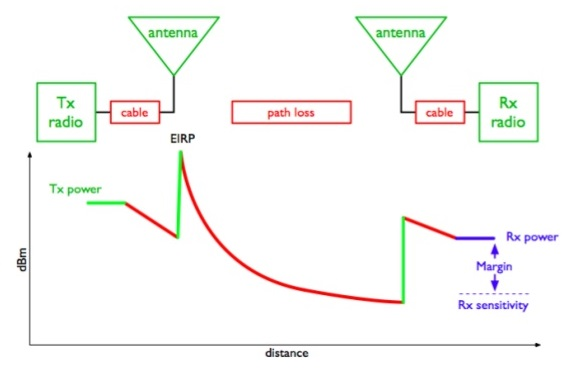
\includegraphics[width=1.0\textwidth]{images/link_budget.jpg}
	\caption{Link Budget}
	\label{img:link_bduget}
\end{figure}
\newpage

\subsection{Frekvencijski pojas}
\label{subsection:lora_freq}
U prethodnim potpoglavljima je spomenut frekvencijski pojas na kojem se odvija komunikacija. Standardne LoRa frekvencije koje ovise o regiji u kojoj se LoRa koristi su: 868 MHz, 915 MHz, 433 MHz i 415 MHz. Navedene frekvencije spadaju u tvz. ISM (eng. Industrial, scientific and medical radio bands) frekvencijski spektar. Iako LoRa primopredajni uređaji mogu raditi na frekvencijama između 137 MHz i 1020 MHz, te tako mogu raditi i na licenciranim frekvencijskim spektrima ipak se najčešće koriste za radu u gore navedenim ISM frekvencijama. Osim frekvencije postoje i definirani pojasevi (eng. bandwidth). U Europi je moguće koristiti pojaseve širine od 125 kHz ili 250 kHz dok je u SADu uz ta dva pojasa dostupan i pojas od 500 kHz.
Na slici \ref{img:bands} specificirani su frekvencijski rasponi, broj kanala u rasponu, maksimalna snaga predajnika i ostali bitni parametri LoRa komunikacije. Potrebno je napomenuti da se rasponi navedenih parametara specificiraju u LoRaWAN standardu (poglavlje \ref{section:lorawan}).

\begin{figure}[ht!]
	\centering
	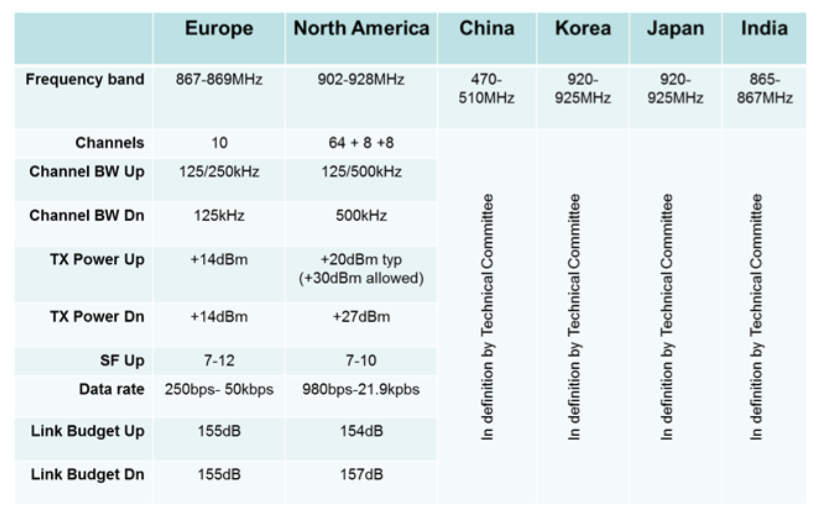
\includegraphics[width=1.0\textwidth]{images/bands.jpg}
	\caption{Parametri komunikacije po regijama}
	\label{img:bands}
\end{figure}

\subsection{LoRa okvir fizičkog sloja}
\label{subsection:lora_frame}
Iako su pojas $BW$ i faktor raspršenja $SF$ varijabilni parametri u LoRa komunikaciji, u pojedinom okviru oni su konstantni. LoRa okvir fizičkog sloja jer varijabilne duljine i započinje preambulom (eng. preamble). Preambula je uzastopni niz upchirp-ova koji pokrivaju cijeli pojas $BW$ i služe kao referenca za postupak demodulacije odnosno za sinkronizaciju prijamnika i predajnika. Zadnja dva upchirp-a predstavljaju sinkronizacijsku riječ zbog koje je moguće razlikovati različite LoRa mreže koje koristi isti frekvencijski pojas. Prijamni LoRa uređaj će prestati 'slušati' ako sinkronizacijska riječ ne odgovara njegovim postavkama. Možemo reći da je sinkronizacijska riječ identifikator mreže. Po završetku sinkronizacijskih chirp-ova slijede 2.25 downchirpa koji označavaju početak polja podataka ili opcionalnog zaglavlja (eng. SFD - Start of Frame Delimiter). Duljina preambule je podesiva i može varirati od 10.25 do 65539.25 simbola. Nakon preambule dolazi zaglavlje (eng. header) koje je opcionalni dio okvira. U zaglavlju se nalaze informacije o: duljini podataka u bajtovima koji se prenose (eng. payload) okvirom, o tome koristi li se CRC i kojim faktorom kodiranja CR su kodirani podaci viših slojeva, koji su enkapsulirani u okvir. Podaci u zaglavlju, ako on postoji, su uvijek kodirani fiksnim faktorom kodiranja $CR = \frac{4}{8}$. Nakon zaglavlja dolazi polje podataka. Polje podataka je limitirano na 255 bajtova jer je duljina polja podatak zapisana jednim bajtom u zaglavlju. LoRa okvir završava opcionalnim CRC poljem. Polje podataka i CRC polje su kodirani CR parametrom definiranim u zaglavlju okvira. Zaglavlje je opcionalno kako bi uštedilo na vremenu slanja (a samim time i na energiji) u slučajevima kada su poznati: duljina podataka, CR i prisutnost CRC polja.
Slika \ref{img:frame} prikazuje format LoRa okvira. na slici \ref{img:chirps_frame} je primjer jednog LoRa okvira u vodopadnom grafu (gdje je horizontalno frekvencija, a vertikalno vrijeme) sa označenim dijelovima. 
\begin{figure}[ht!]
\centering
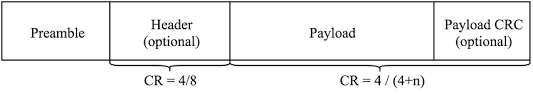
\includegraphics[width=1.0\textwidth]{images/frame.png}
\caption{LoRA okvir fizičkog sloja}
\label{img:frame}
\end{figure}

\begin{figure}[ht!]
\centering
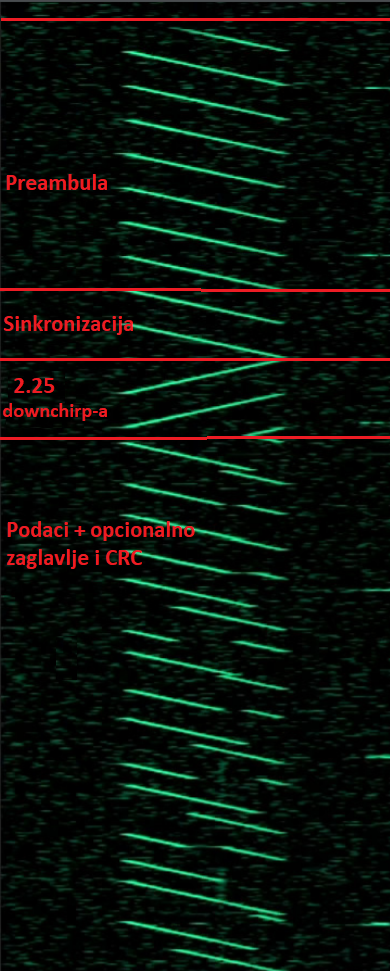
\includegraphics[width=0.4\textwidth]{images/chirps_frame.png}
\caption{Vodopadni prikaz LoRa okvira}
\label{img:chirps_frame}
\end{figure}

\newpage
\subsection{Virtualni kanali}
\label{subsection:lora_virt_channel}
Kako je LoRa modulacija parametrizirana, mijenjanjem parametara moguće je promijeniti karakteristike komunikacijskog kanala te različitim kombinacijama parametara komunikacije postići virtualne kanale.
Virtualni kanali su definirani parovima BW i SF. Iako virtualni kanali koriste isti frekvencijski spektar među njima nema interferencija. Virtualni kanali efektivno povećavaju kapacitet komunikacijskih kanala. Bitno je napomenuti da pojedini virtualni kanali imaju različitu brzinu prijenosa i različit doseg komunikacije (pogledati poglavlje \ref{subsection:lora_mod_params} i relavantne formule). Brzina prijenosa određena je izrazom \ref{eq:r_bit}, a doseg komunikacije osjetljivošću prijamnika koji pak ovisi o parametrima BW i SF.

\subsection{Pouzdanost}
\label{subsection:lora_reliability}
Sam LoRa modulacijski postupak omogućuje robusnost komunikacije tj. otpornost na interferencije. Komunikacija na frekvenciji nižoj od 1 GHz rezultira dobrom penetracijom signala.
LoRa koristi Forward Correction Code (FEC) zbog čega se na strani prijamnika može detektirati i ispraviti greška. Pouzdanost prijenosa podataka može se dodatno optimirati podešavanjem parametara komunikacije (npr. niži BW, veći SF i/ili veći CR). Više o pouzdanosti u radu \cite{pozdanost}.

\newpage
\section{LoRaWAN}
\label{section:lorawan}
LoRaWAN je protokol koji definira kontrolu pristupa komunikacijskom mediju (eng. MAC - Media Access Control) i standard za stvaranje LPWAN mreža baziranih na LoRa tehnologiji.
LoRaWAN definira komunikacijski protokol i arhitekturu mreže oslanjajući se na LoRa tehnologiju obrađenu u poglavlju \ref{section:lora_phy}. Sam protokol i arhitektura mreže imaju izravan utjecaj na trajanje baterije krajnjih uređaja, kapacitet mreže, kvalitetu usluge, sigurnost i druge aspekte bitne za krajnje aplikacije odnosno korisnike LoRa i LoRaWAN tehnologije.
LoRaWAN je dizajnirana primarno za bežične senzorske mreže, ali i druge primjene imajući na umu nekoliko ključnih faktora:
\begin{itemize}
\item Slanje male količine podataka s pojedinog krajnjeg uređaja (čvora)
\item Mala brzina slanja podataka
\item Mala potrošnja energije
\item Kratak period aktivnosti krajnjih uređaja (melen Duty Cycle) - nekoliko poruka dnevno
\item Iznimno velik broj uređaja u mreži - podržava do 1 milijun uređaja
\item Podrška za razne načine rada uređaja - mogučnost optimiranja potrošnje
\item Sigurnost
\end{itemize}
Iako LoRa modulacijski postupak nije otvoreno rješenje, LoRaWAN je otvoreni standard kojeg specificira neprofitna \href{https://lora-alliance.org}{LoRa alijansa}. Glavna zadaća svih članova LoRa alijanse je suradnja na razvoju LoRaWAN standarda. Aktualna verzija LoRaWAN specifikacije je \href{https://lora-alliance.org/resource-hub/lorawantm-specification-v11}{1.1}
\newline

Bitno je napomenuti da je moguće koristiti LoRa tehnologiju i bez LoRaWAN protokola. Međutim, LoRaWAN je široko prihvaćen otvoreni standard i takva situacija nije česta. Na primjer, možemo koristiti LoRu bez LoRaWAN protokola kada želimo ostvariti vezu između samo dva LoRa primopredajnika (peer-to-peer).
        
\subsection{Arhitektura mreže}
\label{subsection:lorawan_network_arh}
LoRaWAN koristi zvijezdastu topologiju mreže. Svaki krajnji uređaj u mreži može komunicirati (bidirekcionalno) sa više LoRa premosnika (eng. LoRa gateway). Dakle, krajnji uređaj nema definiran vlastiti premosnik već se okviri šalju svim premosnicima (eng. Broadcast). S obzirom da u mreži može biti više premosnika povezanih na mrežni server, a sa svakim premosnikom može biti povezano više krajnjih uređaja, često se kaže da LoRaWAN ima dvostruku zvijezdastu topologiju (eng. Star of Stars).
\begin{figure}[ht!]
	\centering
	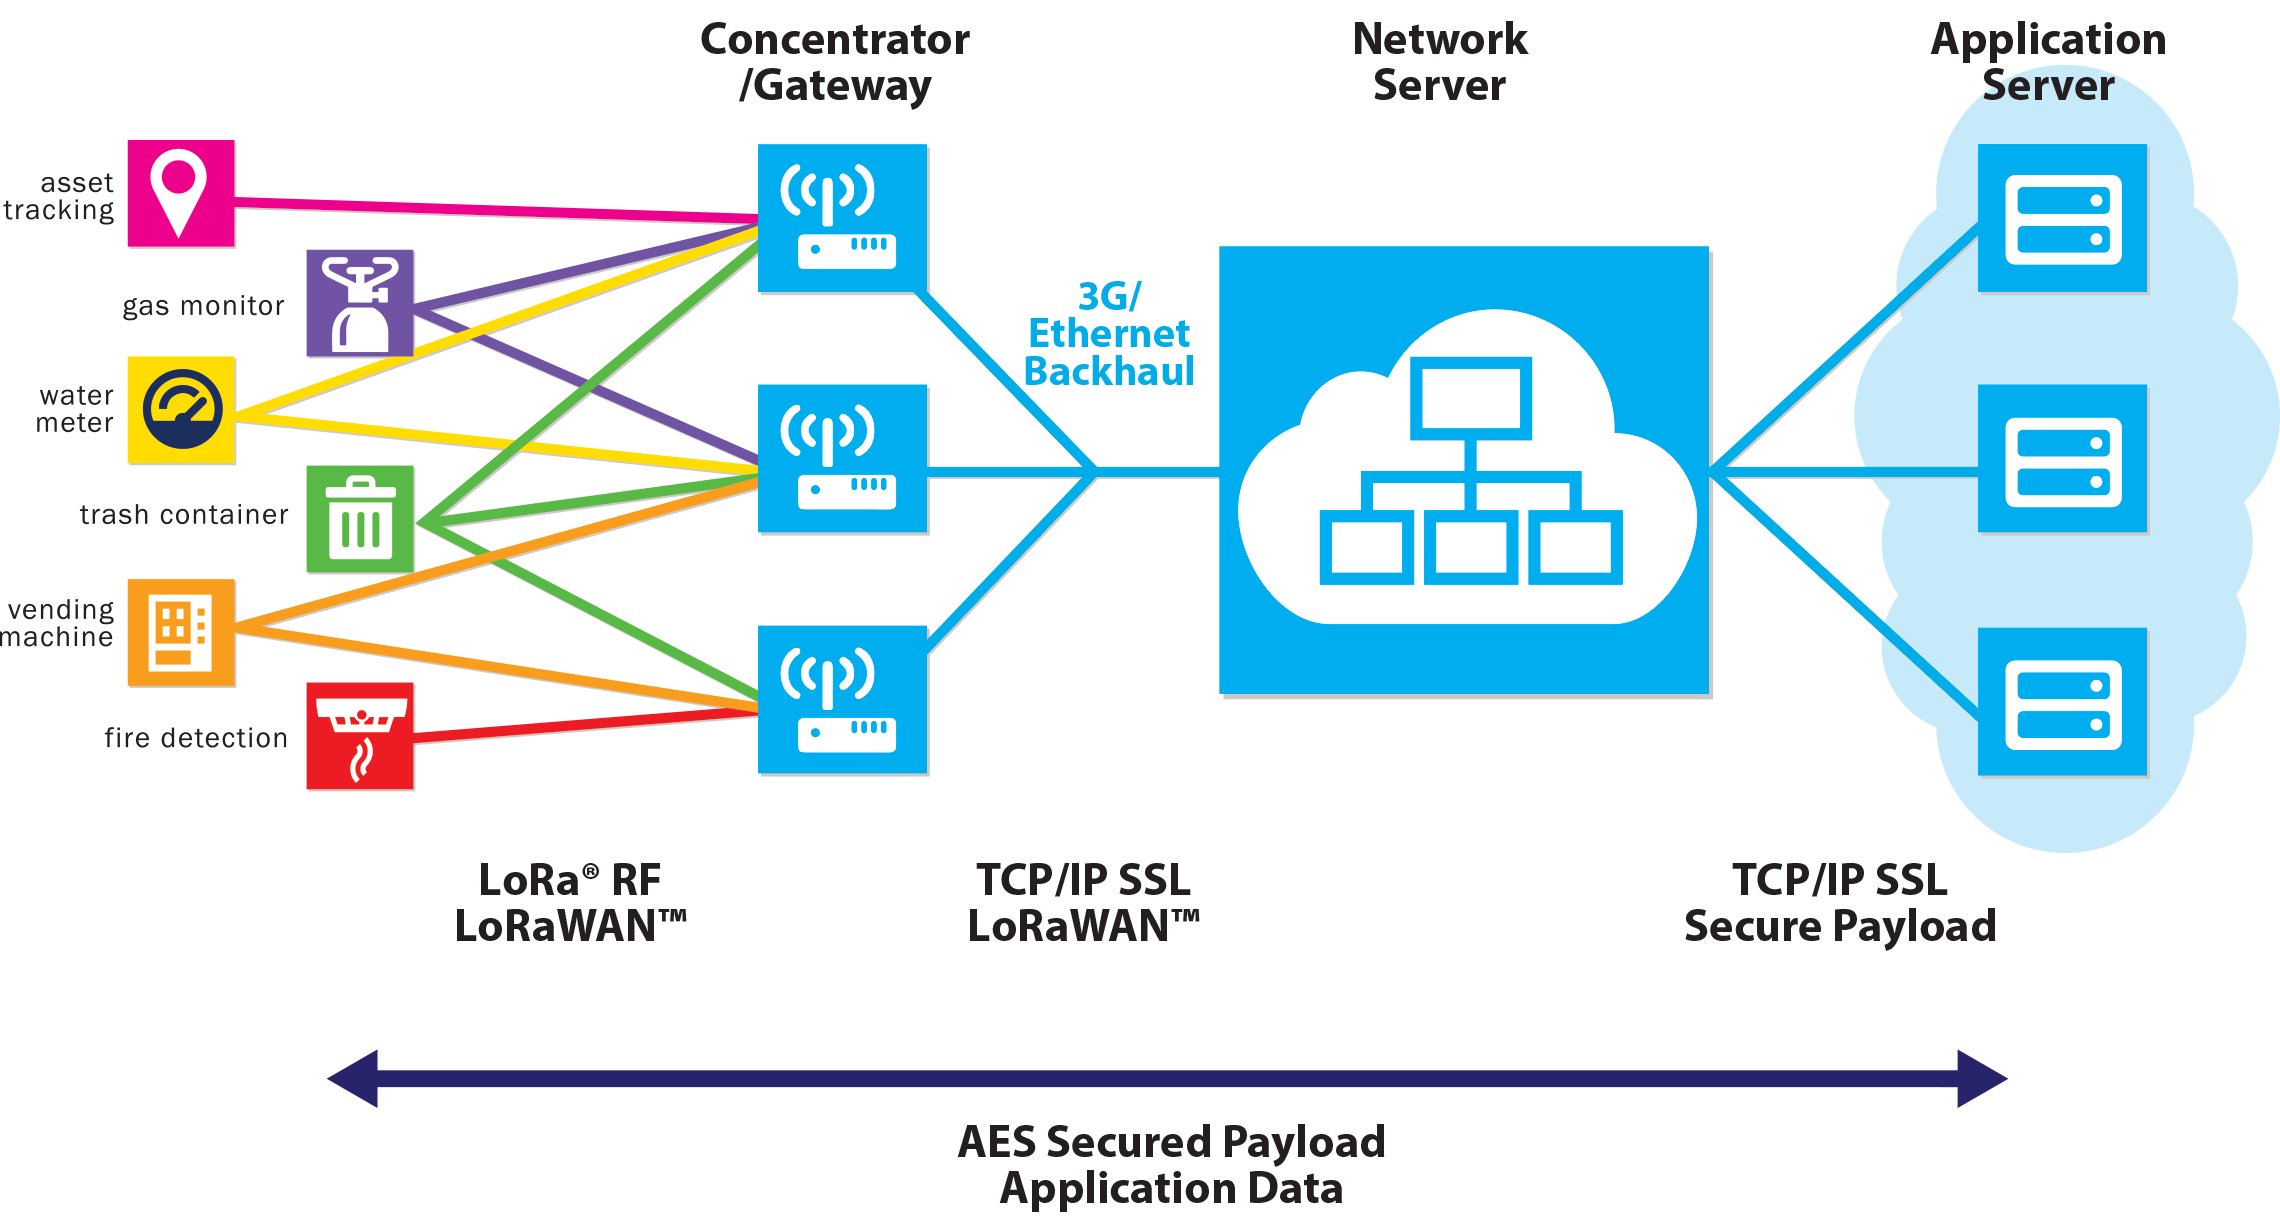
\includegraphics[width=1.0\textwidth]{images/lorawan_network.png}
	\caption{Topologija LoRaWAN mreže}
	\label{img:bands}
\end{figure}

\subsection{Komponente LoRaWAN mreže}
\label{subsection:lorawan_components}
LoRaWAN specifikacija definira nekoliko komponenti potrebnih za ostvarenje LoRaWAN mreže:
\begin{itemize}
\item \textbf{Krajnji LoRa uređaj} - uređaj male potrošnje električne energije, opremljen senzorima i/ili aktuatorima, komunicira s premosnicima

\item \textbf{LoRa premosnik} (eng. Gateway) - prosljeđuje pakete primljene od krajnjih uređaja prema mrežnom poslužitelju i obrnuto. Komunikacijsko sučelje prema krajnjim uređajima je LoRa, a prema mrežnom poslužitelju IP (npr. Ethernet ili 4G) što omogućuje veliku propusnost prema mrežnom poslužitelju koja je nužna zbog velikog broja krajnjih uređaja. Više premosnika može primiti isti paket, ali ga svi prosljeđuju prema mrežnom poslužitelju. Premosnik dodaje podatke o kvaliteti signala. Premosnik se također brine o vremenskim intervalima unutar kojih se paketi šalju prema krajnjim uređajima tj. brine se o sinkronizaciji s krajnjim uređajima.

\item \textbf{LoRa mrežni poslužitelj} - ostvaruje stalnu vezu s premosnicima i prosljeđuje poruke odgovarajućim aplikacijskim poslužiteljima. Obavlja agregaciju primljenih paketa i odbacuje duplikate primljenih paketa. Stvara ACK poruku za poruke koje zahtjevaju potvrdu. Zaprima poruke od aplikacija, generira pakete koji se šalju prema krajnjim uređajima i prosljeđuje ih premosnicima. Odlučuje koji će premosnik odgovoriti krajnjem uređaju tako što prati parametre komunikacije odnosno kvalitetu pojedine veze u mreži (eng. RSSI - Received Signal Strength Indication). Mrežni poslužitelj upravlja mrežom i krajnjim uređajima slanjem MAC naredbi. Možemo reći da je kompleksnost LoRaWAN protokola najvećim dijelom sadržana u mrežnom poslužitelju što je i logično ako se želi uštediti energija na krajnjim uređajima.

\item \textbf{Aplikacijski poslužitelj} - prikuplja i analizira podatke i šalje poruke prema krajnjim uređajima preko ostatka mreže. Ujedno veza između korisničke aplikacije i LoRa poslužitelja.
\end{itemize}

\subsection{Klase uređaja}
\label{subection:classes}
LoRaWAN specifikacija definira tri klase krajnjih uređaja odnosno tri načina rada. Svi krajnji uređaji moraju implementirati klasu A, a klasa B i C su proširenja na specifikaciju klase A.
\begin{itemize}
\item \textbf{Klasa A} - energetski najštedljivija, ograničeno bi-direkcionalna (nepoznata latencija)

U klasi A komunikaciju uvijek iniciraju krajni uređaji i potpuno je asinkrona. Komunikacija od krajnjih uređaja prema premosnicima može biti pokrenuta u bilo kojem trenutku. Nakon uplink komunikacije slijede, s vremenskim odmakom (RxDelay), 2 prozora (RX1 i RX2) unutar kojih se može odviti downlink komunikacija tj. slanje prema krajnjim uređajima. Poruke sa poslužitelja u bilo kojem drugom trenutku moraju pričekati da krajni uređaj inicira komunikaciju kako bi u idućem downlink prozoru mogli poslati svoje poruke. Drugim riječima downlink komunikacija ovisi o uplink komunikaciji pa je nepoznata downlink latencija, ali ipak postoji mogučnost bi-direkcionalne komunikacije.
\begin{figure}[ht!]
	\centering
	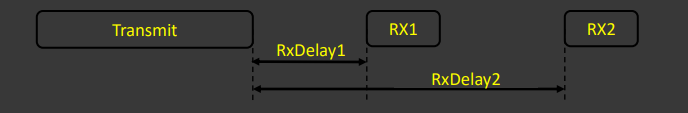
\includegraphics[width=0.9\textwidth]{images/a_class.png}
	\caption{Klasa A}
	\label{img:class_a}
\end{figure}
\newpage
\item \textbf{Klasa B} - bi-direkcionalna komunikacija sa poznatom latencijom, malo veća potrošnja energije

Klasa B je proširenje klase A gdje su uređaji u mreži sinkronizirani tzv. periodičkim \textit{beacon} signalom kojeg postavlja premosnik. U klasi B postoje dodatni downlink prozori (tzv. ping slot) u periodičkim trenucima. Premosnici znaju trenutke u kojima krajnji uređaji slušaju te tada mogu obaviti slanje paketa prema krajnjim uređajima. Latencija je deterministička i podesiva do 128 sekundi kako bi se komunikacija mogla prilagoditi raznim aplikacijama, a da se zadrži mala potrošnja energije.
\begin{figure}[ht!]
	\centering
	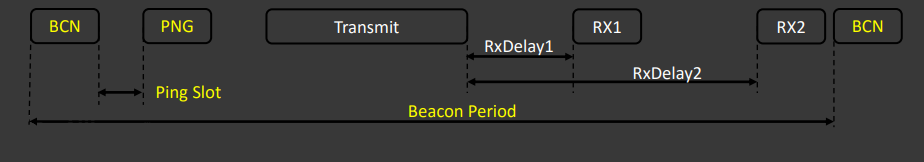
\includegraphics[width=0.9\textwidth]{images/b_class.png}
	\caption{Klasa B}
	\label{img:class_b}
\end{figure}
\item \textbf{Klasa C} - najmanja latencija (praktički Half-Duplex komunikacija), najveća potrošnja energije

Proširenje klase A: nakon uplink komunikacije tj. slanja od krajnjeg uređaja prema premosnicima i isteka vremenskog perioda RxDelay, krajnji uređaj nastavlja slušati sve do slijedećeg slanja prema premosnicima. Nedostatak klase C je iznimno velika potrošnja energije ako ju usporedimo s klasom A i B.

\begin{figure}[ht!]
	\centering
	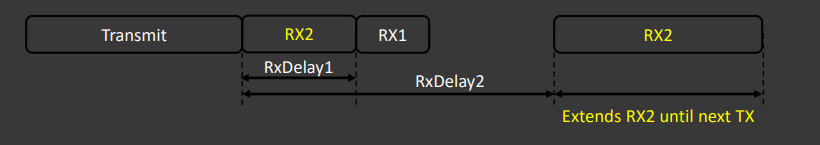
\includegraphics[width=0.9\textwidth]{images/c_class.png}
	\caption{Klasa C}
	\label{img:class_c}
\end{figure}
\end{itemize}

\subsection{Adaptive Data Rate (ADR)}
Kako bi se maksimiziralo trajanje baterije krajnjih uređaja i kapacitet mreže, a ostvarila potrebna brzina i doseg komunikacije, LoRaWAN mrežni poslužitelj upravlja postavkom DR (Data Rate) i izračenom RF snagom krajnjih uređaja. Postavka DR je izravno povezana s parametrima SF i BW. LoRa premosnici optimiraju mrežu tako što iskorištavaju svojstvo da na istom frekvencijskom rasponu BW mogu istovremeno primati podatke ako oni dolaze drugačijim parametrom SF (pogledati potpoglavlje o virtualnim kanalima \ref{subsection:lora_virt_channel}). Brzine prijenosa u LoRaWAN mreži variraju između nekoliko bps do 50kbps za isti parametar BW.

\subsection{Kapacitet mreže}
Visok kapacitet mreže potreban je zbog velikog broja krajnjih uređaja koji komuniciraju s premosnicima. Kapacitet mreže ključna je osobina mreže bitna za performanse i skalabilnost same mreže. Visok kapacitet u LoRaWAN mreži je osim podesivim parametrom DR ostvaren i višestrukim komunikacijskim kanalima.
\begin{figure}[ht!]
	\centering
	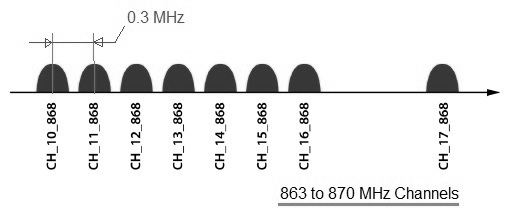
\includegraphics[width=0.9\textwidth]{images/lora_channels.jpg}
	\caption{Kanali LoRa 868MHz spektra (EU)}
	\label{img:channels}
\end{figure}
LoRa premosnici su dizajnirani tako da istovremeno mogu primati poruke na više kanala (eng. Multichannel i Multimodem), a još k tome na svakom fizičkom kanalu postoje virtualni kanali što efektivno dodatno povečava kapacitet mreže.

\subsection{Format LoRaWAN poruke}
\label{subsection:lorawan_packet}
LoRaWAN poruka se enkapsulira u LoRa fizički okvir opisan u potpoglavlju \ref{subsection:lora_frame}. Format LoRaWAN paketa prikazan je na slijedećoj slici.
\begin{figure}[ht!]
	\centering
	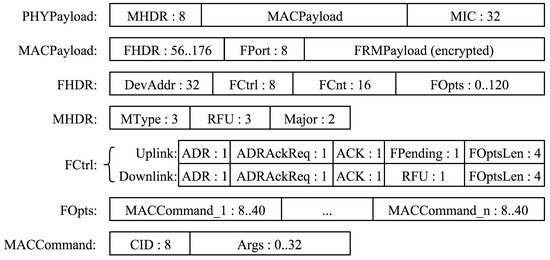
\includegraphics[width=0.9\textwidth]{images/packet.jpg}
	\caption{LoRaWAN paket}
	\label{img:lorawan_packet}
\end{figure}

\newpage
Polja LoRaWAN poruke:
\begin{itemize}
\item MHDR (MAC header) - definira tip poruke
\item MACPayload - podaci LoRaWAN poruke (sastoji se od zaglavlja okvira(FHDR), podataka okvira (FRMPayload) i porta FPort)
\item MIC (Message Integrity Code) - osigurava integritet poruke
\item DevAddr - kratka adresa uređaja
\item FPort - ako je vrijednost 0, radi se o MAC naredbi
\item FRMPayload - korisni podaci okvira kriptirani 128 bitnim AES ključem
\item FCtrl - kontrolni oktet
\begin{itemize}
\item FOptsLen - duljina FOpts polja - 0 ako se radi o MAC naredbi
\item vrsta poruke (uplink ili downlink)
\item ACK - zahtjev za potvrdom
\item ADR - podesivi Data Rate
\item FPending - oznaka da postoji još podataka za slanje (samo u downlink porukama)
\end{itemize} 
\item FCnt - brojač okvira
\item FOpts služi za prijenos MAC naredbi  u podatkovnoj poruci, ako postoji, polje FOpts je kriptirano NwkSEncKey ključem (ključem enkripcije na razini mreže).
\end{itemize}

\subsection{Integriranje krajnjeg uređaja u LoRaWAN mrežu}
\label{subsection:end_node_integration}
Kako bi sudjelovao u LoRaWAN mreži, krajnji uređaj mora biti aktiviran. Dostupna su dva načina aktivacije krajnjih uređaja: OTAA (Over-The-Air Activation) i ABP (Activation By Personalization):
\begin{itemize}
\item OTTA - Procedura aktivacije kod koje se koriste zahtjevi za pristup (eng. join-request) i odgovori na zahtjeve za pristup (eng. join-accept) mreži. Ovisno o odgovoru na zathjev, krajnji uređaj mogu dobiti ključeve za novu mrežnu i aplikacijsku sesiju.
\item ABP - ključevi za sesiju su izravno upisani u krajnje uređaje
\end{itemize}
Svakom krajnjem uređaju potrebne su slijedeće informacije kako bi se mogao integrirati u mrežu:
\begin{itemize}
\item Adresa krajnjeg uređaja (DevAddr) - 32-bitni identifikator krajnjeg uređaja, 7 bitova je identifikator mreže, a preostali identifikator uređaja
\item Identifikator AppEUI - globalni identifikator iz IEEE EUI64 adresnog prostora koji jedinstveno identificira krajnji uređaj
\item Ključ mrežne sesije (NwkSKey) - ključ korišten od strane mrežnog poslužitelja i krajnjeg uređaja u svrhu verficiranja integriteta poruke i autentifikacije uređaja
\item Ključ aplikacijske sesije (AppSKey) - ključ korišten od strane mrežnog poslužitelja i krajnjeg uređaja u svrhu kriptiranja i dekriptiranja korisnih podataka u poruci
\end{itemize}

\subsection{Sigurnost}
\label{subsection:security}
Iznimno je bitno za svaku LPWAN mrežu pa tako i za LoRaWAN da implementira sigurnost.
LoraWAN protokol sadrži sigurnost u dva sloja: jedan sloj sigurnosti za mrežu (NwkSKey ključ) i jedan sloj za aplikaciju (AppSKey ključ). Mrežni sloj sigurnosti se brine za autentifikaciju kranjeg uređaja (kriptiranjem poruke), a aplikacijski sloj sigurnosti osigurava kontrolu pristupa aplikacijskim podacima (kriptiranjem podataka AES enkripcijom).

\begin{figure}[ht!]
	\centering
	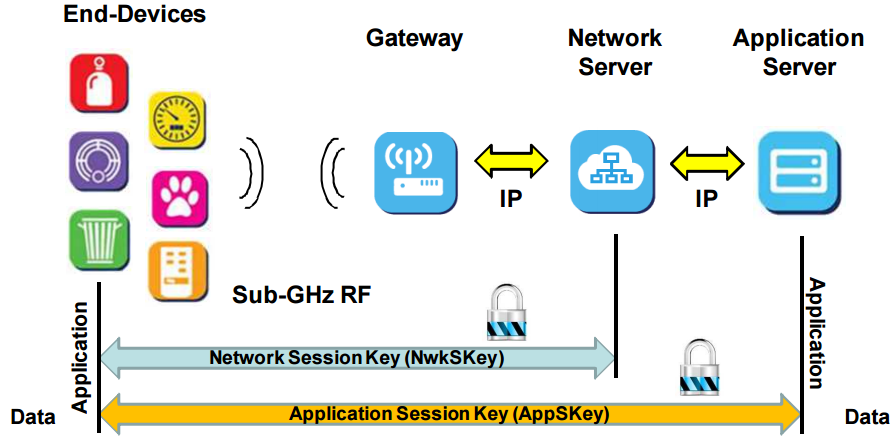
\includegraphics[width=0.9\textwidth]{images/security.png}
	\caption{Slojevitost sigurnosti LoRaWAN protokola}
	\label{img:security}
\end{figure}
\chapter{Zaključak}
\label{chapter:uvod}

Mnoge analize predviđaju da će do 2020. godine na internet biti spojeno preko 50 milijardi uređaja od ćega preko 20 milijardi uređaja putem LPWAN mreža. Potreba za LPWAN tehnologijama je sve veća. LoRa i LoRaWAN su jedna od mogučih tehnologija. Po mnogim karakteristikama LoRa je optimalan izbor. Vrijeme i masovnija analiza i primjena ovih tehnologija pokazat će prednosti i mene pojedine tehnologije, a možda i izum neke nove.

\bibliography{literatura}
\bibliographystyle{fer}
\nocite{lora_app_note}

\begin{sazetak}
U uvodnom dijelu dane su osnovne informacije o tome što je LPWAN, odnosno o mreži širokog raspona i male potrošnje energije. Navedene su osnovne karakteristike i primjene LPWAN tehnologija. U uvodu je također spomenuta i LoRa kao jedna od mogučih tehnologija za ostvaranje takve mreže te ostale prisutne tehnologije. U nastavku rada detaljnije je opisana LoRa tehnologija i njezine karakteristike, mogučnosti i ograničenja. U zadnjem dijelu rada ukratko je razrađen  LoRaWAN protokol i opisana pripadna arhitektura LoRaWAN mreže.
\newline
\linebreak
\kljucnerijeci{LPWAN; LoRa; LoRaWAN; LoRa Alliance; Semtech; IoT; Internet Of Things; M2M}
\end{sazetak}

\end{document}
